\documentclass[10pt]{article}
\usepackage{fancyhdr}
\usepackage{hyperref}
\usepackage{dirtree}
\usepackage[margin=0.6in]{geometry}
\usepackage{graphicx} 


\hypersetup{
    colorlinks=true,
    linkcolor=blue,
    urlcolor=blue,
}


\title{ANGRY BIRDS \\ 2\_PLAYERGAME }
\author{Maradana Sai Siva Lochan }
\date{Spring 2024-2025}

\pagestyle{fancy}
\lhead{ANGRY\_BIRDS}
\rhead{Lochan}

\begin{document}

    \maketitle

    \begin{abstract}
        This report outlines the development process of creating the game: Angry Birds: Two-Player Showdown, a 2D physics-based projectile game built using Python and Pygame.
        It covers the game’s concept, mechanics, design, implementation structure, and the challenges encountered throughout development..
    \end{abstract}

    \tableofcontents
    \newpage


    \section{Introduction}
    The aim of this game is to destroy the opposing player's block structures using physics-based projectiles. Each player takes turns launching birds from their respective catapults, attempting to inflict maximum damage on the opponent’s defense.

    Victory is based on strategic aim, timing, and efficient destruction. While no traditional score counter exists, performance can be measured by factors such as number of successful hits, remaining blocks, or number of turns taken to dismantle the opponent's setup.


    \section{Modules}\label{sec:modules}
    The external modules used are:
    \begin{itemize}
        \item \texttt{pygame} - pygame is a set of Python modules designed for writing video games.
        \item \texttt{Random} - A module that implements pseudo-random number generators for various distributions.
        \item \texttt{Sys} - A module that provides access to some variables used or maintained by the interpreter and to functions that interact with the interpreter.
        \item \texttt{Time} - A module that provides various time-related functions.
        \item \texttt{os} - A module that provides a portable way of using operating system-dependent functionality.
        \item \texttt{math} - A module that provides access to mathematical functions such as trigonometry, logarithms, exponentials, and constants like $\pi$. It was used to handle vector calculations and angle measurements in projectile motion and collision handling.
    \end{itemize}


    \section{Directory Structure}
    The project directory has:

    \begin{enumerate}
        \item{menu.py}
        \item {main.py}
        \item {blocks.py}
        \item {angry\_birds.py}
        \item {projectiles.py}
        \item {Images}
    \end{enumerate}



    \begin{itemize}
        \item \textbf{main.py} - Manages the start menu interface, player name input, and transition into the game and it will start game by running 
        \item \textbf{game.py} - Controls the core game loop, player switching, bird launching, collision handling, and game state transitions.
        \item \textbf{blocks.py} - Defines the Block class and handles the drawing, positioning, health bar, and falling animation of block structures.
        \item \textbf{angry\_birds.py} - loads bird images and sets their initial positions and display on screen.
        \item \textbf{projectiles.py} - Manages projectile (bird) behavior including physics (velocity, gravity), movement updates, and collision side detection.
        \item \textbf{Images} - contains all images related to the game
    \end{itemize}


    \section{Running Instructions and Prerepuisites}

    install python first\\
    Now install \texttt{pygame} by using command 
    "\texttt{pip install pygame}"\\
    The file can be run by: \\
    \texttt{python main.py } \\
    \texttt{python3 main.py } \\

    \section{Game Play!}
    \subsection{Game Navigation }
    use play button to move from intro screen to main menu and also main menu to game play screen OR you may use enter keys

    \subsubsection{Intro Screen}
    The game starts with an Intro Screen[\ref{fig:Intro}]:
    \begin{figure}[h!]
        \centering
        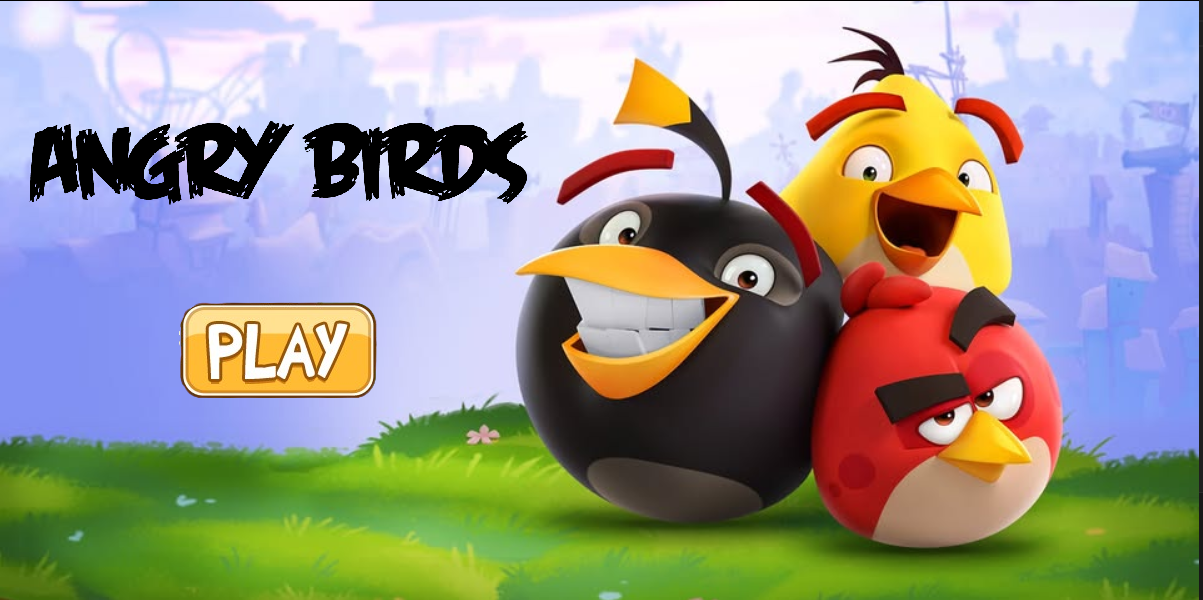
\includegraphics[width=0.5\textwidth]{Intro}
        \caption{Intro Screen}\label{fig:Intro}
    \end{figure}

    \subsubsection{Main Menu}
    Here we need to fill the names of the players (2 players) before we choose to play \\
    We can select any of these by pressing on these\\
    We can also use key down or upper arrows or enter key to
    navigate[\ref{fig:MainMenu}].
    \begin{figure}[h!]
        \centering
        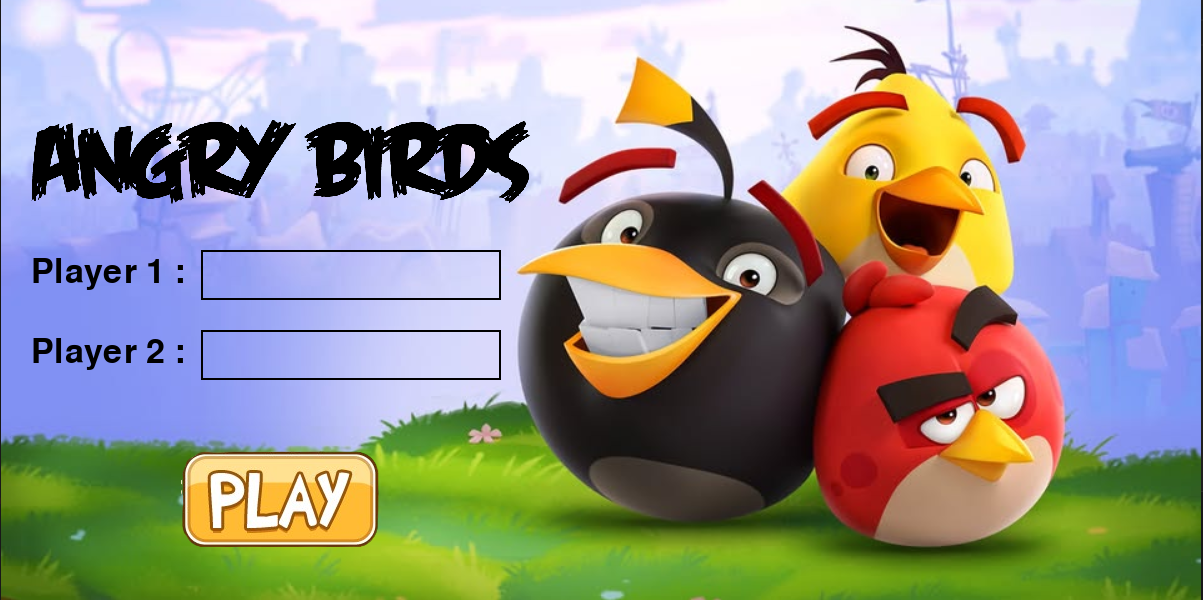
\includegraphics[width=0.5\textwidth]{MainMenu}
        \caption{Main Menu}\label{fig:MainMenu}
    \end{figure}
    \newpage
    \subsubsection{The Game!}
    \begin{itemize}
        \item The game is designed for \textbf{two players}, each taking alternate turns.
        \item On a player's turn, they can \textbf{select one bird} from the available options and \textbf{drag it using the mouse} from their catapult to adjust angle and power.
        \item Upon releasing the mouse, the bird is launched and follows a realistic \textbf{projectile trajectory} with gravity and collisions.
        \item The bird can bounce off blocks depending on which side of the block it hits.
        \item The objective is to \textbf{hit and destroy the opponent’s block structures}.
    \end{itemize}
    Some examples of the game screens[\ref{fig:GameStart}][\ref{fig:GamePlay}].
    \begin{figure}[h!]
        \centering
        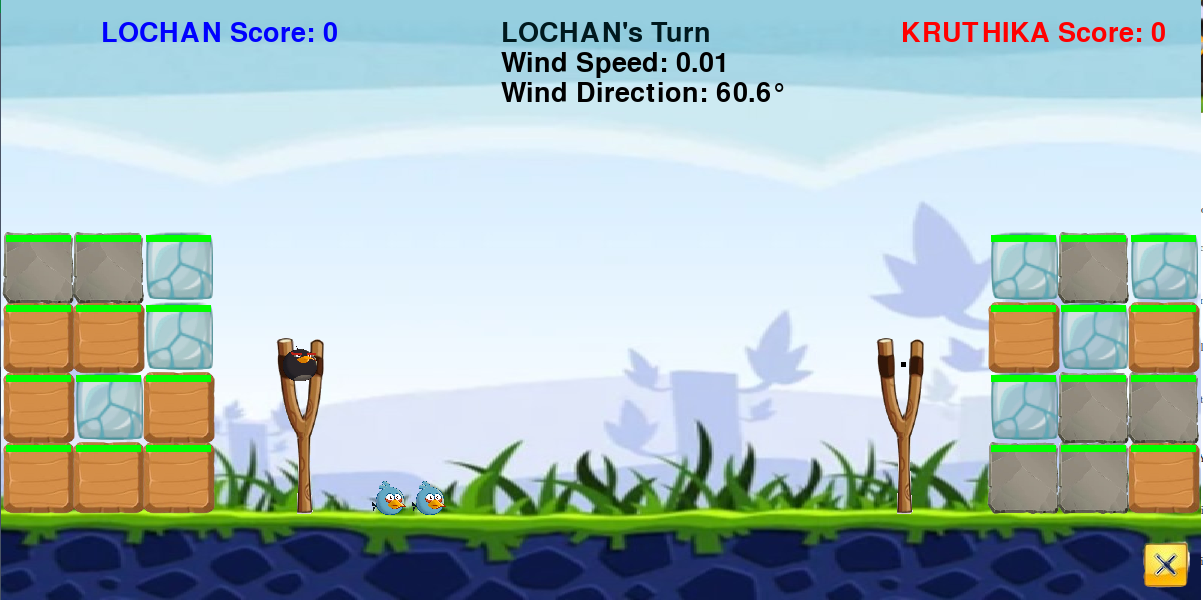
\includegraphics[width=0.5\textwidth]{GameStart}
        \caption{Game Starts!}\label{fig:GameStart}
    \end{figure}\\
    NOTE\\
    \begin{itemize}
    \item Each player may launch one bird per turn.
    \item Blocks have a defined \textbf{health level}, which decreases on each hit.
    \item When the bird hits block then it reflects and falls down and goes out of screen,Here ground collision is not considered
    \item The game continues with alternating turns until a victory condition is met (e.g., one player’s blocks are all destroyed).
    \item There is no formal score system; performance can be judged based on \textbf{number of hits}, \textbf{remaining structures}, or \textbf{efficiency}.
    \end{itemize}
    \begin{figure}[h!]
        \centering
        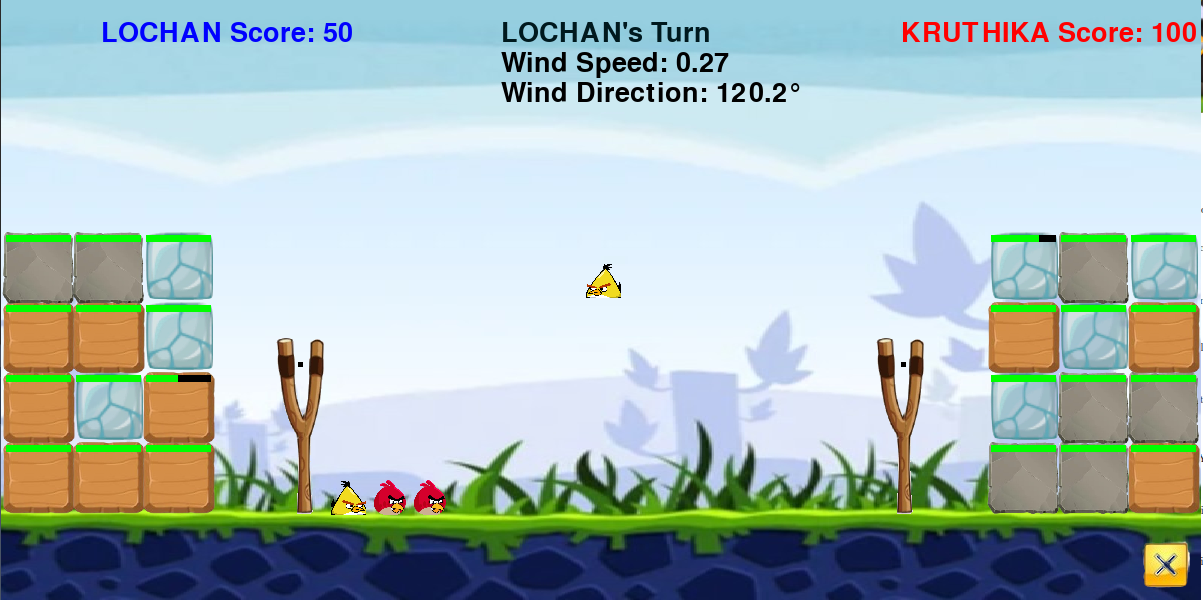
\includegraphics[width=0.5\textwidth]{GamePlay}
        \caption{ Game Play!}\label{fig:GamePlay}
    \end{figure}

    \subsubsection{Game Over}
    The game ends when all blocks on one side are completely destroyed, declaring the opposing player as the winner.\\
    We can also end the game in between, Then the player with hight score is considered as the winner
    The screen looks like this[\ref{fig:GameOver}]:
    \begin{figure}[h!]
        \centering
        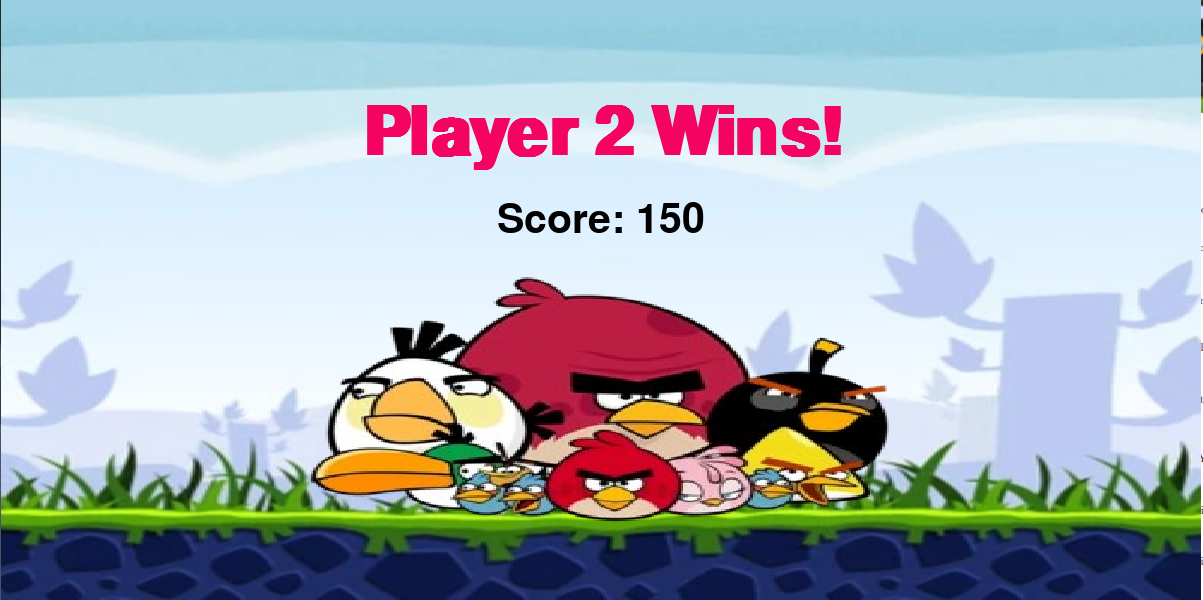
\includegraphics[width=0.5\textwidth]{GameOver}
        \caption{Game Over}\label{fig:GameOver}
    \end{figure}

    Here a low varing wind will always blow and the angle of wind also varies over 360 degrees[\ref{fig:Wind}]:
    \begin{figure}[h!]
        \centering
        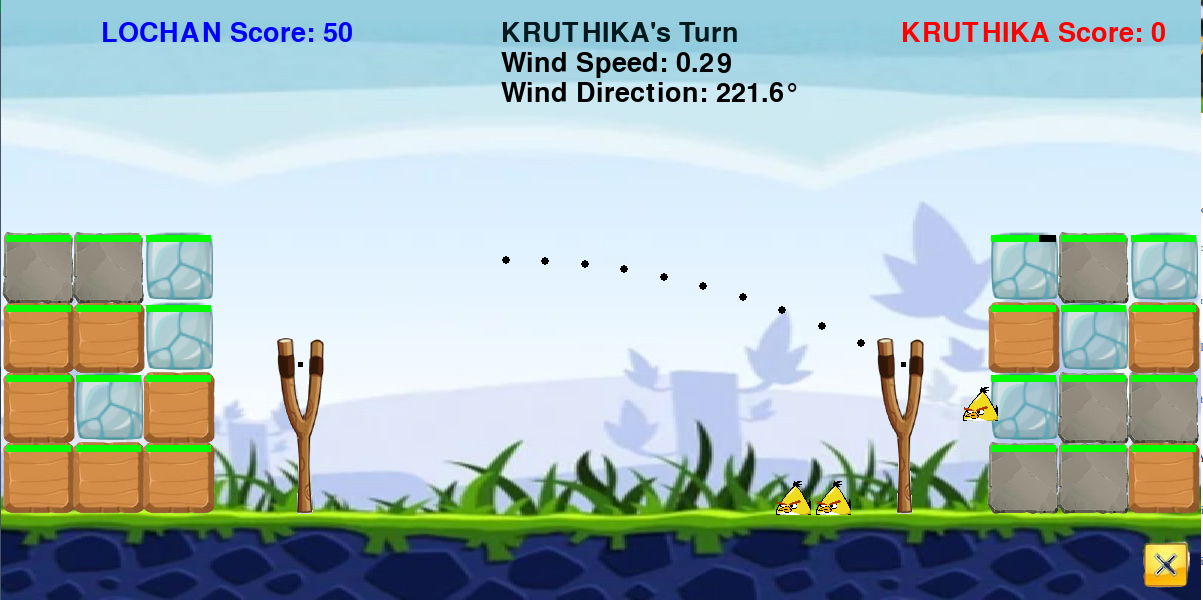
\includegraphics[width=0.5\textwidth]{Wind}
        \caption{Fastest Solves}\label{fig:Wind}
    \end{figure}


    \subsubsection{Quit}
    On clicking this \texttt{X} button, the Game ends and the program terminates.


    \section{My Code}\label{sec:implementation}

The game was developed using Python and the \texttt{pygame} module, which enables real-time rendering, event handling, and sprite manipulation for interactive 2D games. The implementation centers around modular Python files, each handling a core part of the game logic.

To simulate realistic projectile motion, I used \texttt{pygame.math.Vector2} for velocity and direction vectors. Gravity is applied frame-by-frame, updating the vertical velocity of projectiles over time. When a projectile hits a block, the side of collision is detected using bounding box overlap, and its velocity vector is reflected accordingly to simulate bouncing.

Blocks have individual health bars, and when a block’s health reaches zero, it is marked as destroyed.

The game uses mouse event tracking for drag-and-release aiming, switching turns between two players after each bird launch.

Throughout development, I frequently referred to the \texttt{pygame}  documentation\cite{pygame}. 


    \subsection{Customization in the Game}\label{subsec:customisations-in-the-game}
    A list of all the special customization implemented in the game:
    \begin{itemize}
        \item Scores.
        \item Wind
        \item exit Button for easy navigation.
        \item enter keys usage
    \end{itemize}



    \begin{thebibliography}{5}
        \bibitem{pygame}
        Pygame Official Documentation\
        \url{https://www.pygame.org/docs/}.
        \bibitem{angry_birds1}
        Real angry birds game (I)(by professer)\
        \url{https://github.com/estevaofon/angry-birds-python}
        \bibitem{angry_birds2}
        Real angry birds game (II)(by professer)\
        \url{https://github.com/marblexu/PythonAngryBirds}

    \end{thebibliography}

\end{document}